\documentclass[twocolumn]{article}
% Fonts and typesetting settings
\usepackage[sc]{mathpazo}
\usepackage[T1]{fontenc}
\linespread{1.05} % Palatino needs more space between lines
\usepackage{microtype}
% Page layout
\usepackage[hmarginratio=1:1,top=32mm,columnsep=20pt]{geometry}
\usepackage[font=it]{caption}
\usepackage{paralist}
% Lettrines
\usepackage{lettrine}
% Abstract
\usepackage{abstract}
	\renewcommand{\abstractnamefont}{\normalfont\bfseries}
	\renewcommand{\abstracttextfont}{\normalfont\small\itshape}
% Titling (section/subsection)
\usepackage{titlesec}
\renewcommand\thesection{\Roman{section}}
\titleformat{\section}[block]{\large\scshape\centering}{\thesection.}{1em}{}
% Math Packages
\usepackage{amsmath}
\usepackage{amsfonts}
\usepackage{amssymb}
\newcommand{\xor}{\oplus}
% Header/footer
\usepackage{fancyhdr}
	\pagestyle{fancy}
	\fancyhead{}
	\fancyfoot{}
	\fancyhead[C]{Introduction to Cryptographic Algorithms $\bullet$ Assignment: Short Paper}
%including sourcecode in text
\usepackage{verbatim}

% ------
% Clickable URLs (optional)
\usepackage{hyperref}
% ------
% Maketitle metadata
\title{\vspace{-15mm}%
	\fontsize{24pt}{10pt}\selectfont
	\textbf{Review of:\\Plaintext Recovery Attacks against SSH}
	}	
\author{%
	\large
	\textsc{Raoul Estourgie} \\[2mm]
	\normalsize	Radboud University Nijmegen \\
	\normalsize	s3022420
	\vspace{-5mm}
	\and 
	\large
	\textsc{Ben Br\"ucker} \\[2mm]
	\normalsize	Radboud University Nijmegen \\
	\normalsize	s0413291
	\vspace{-5mm}
	}
\date{}
\bibliographystyle{ieeetran}
\usepackage[pdftex]{graphicx}
%%%%%%%%%%%%%%%%%%%%%%%%


\begin{document}

\twocolumn[\begin{@twocolumnfalse}
  \maketitle
  \begin{abstract}
  \noindent This is a review/summary of the article "Plaintext Recovery Attacks against SSH" by Martin R. Albrecht, Kenneth G. Paterson and Gaven J. Watson~\cite{Albrecht2009}. We discuss their findings concerning a possible attack on the OpenSSH implementation of the SSH BPP protocol. This attack enables an attacker to recover 14 bits of plaintext with probability $2^{-14}$ and 32 bits with probability $2^{-18}$. We also cover their suggestions for preventing thse attacks.
\end{abstract}
\end{@twocolumnfalse}]

\thispagestyle{fancy}

\lettrine[nindent=0em,lines=3]{S} ecure Shell (SSH) connects computers securely over insecure network connections~\cite{Ylonen2006}. This protocol was released in 1995 and was designed to replace rlogin, rsh, Telnet and similar insecure protocols. 
\indent The SSH protocol covers authentication, confidentiality and integrity~\cite{Barret2001}.
\indent Our review article "Plaintext Recovery Attacks against SSH" paper~\cite{Albrecht2009} focuses their attack on the OpenSSH implementation of the SSH Binary Packet Protocol (BPP).

\section{The SSH-BPP protocol}
\indent The Binary Packet Protocol (BPP) of SSH encrypts a plaintext and then protects it's integrity by appending a MAC value~\cite{Ylonen2006}.

\indent Before encryption, the message is encoded by prefixing a 4 byte packet-length field and a 1 byte padding-length field. At least 4 bytes of randomized padding must be added as a suffix with a maximum of 255 bytes~\cite{Albrecht2009}. The message is then encrypted with a cypher of choice, for example aes128-cbc. After that, a MAC value is added. This MAC is computed from the cyphertext and a 32-bit packet sequence number. (See figure ~\ref{fig:BPPProtocol})

\indent The packets then form a data stream since the encryption is in CBC mode. Every packet $i-1$ on a connection will be the initialization vector (IV) for packet $i$ on the same connection~\cite{Albrecht2009}.

\indent For decryption it is essential that the receiver decrypts the first ciphertext block to be able to read the length field. Without this he does not know when a complete packet has arrived and when to perform the MAC check. Most SSH implementations wait for a time until enough data has arrived to complete the packet~\cite{Albrecht2009}.

\indent The SSH protocol~\cite{Ylonen2006} also specifies error handling for the BPP protocol. The connection should terminate whenever a transmission error occurs or MAC verification fails. When such a termination happens,the connection should be re-established. Implementations are free to send error messages to their peer when an error occurs.

\begin{figure*}
	  \centering
    	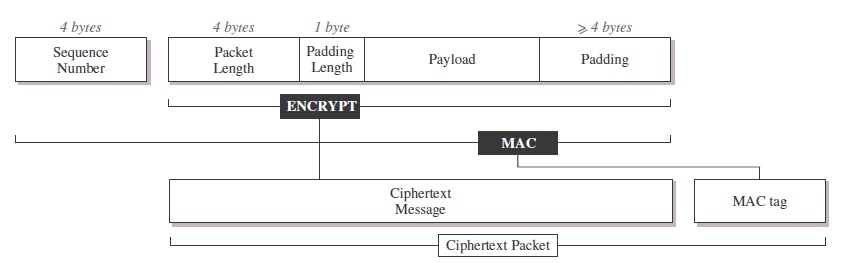
\includegraphics[scale=.6]{SSHBPP.png}
	\caption{SSH BPP packet format and cryptographic processing~\cite{Albrecht2009}}
	\label{fig:BPPProtocol}
\end{figure*}

\section{Open SSH implementation of the BPP protocol}

\indent Open SSH follows the guidelines for BPP fairly close~\cite{Albrecht2009}. But the details about the specific implementation are important, since these details enable the attack by Albrecht et al.~\cite{Albrecht2009}.

\indent After receiving the first ciphertext block, Open SSH first performs a length check. If the length given in the length field is not between 5 and $2^{18}$ it sends a \textit{SSH2 MSG DISCONNECTED} error back to the sender.

\indent Next OpenSSH checks that the total number of bytes expected is indeed a multiple of the block size. When this check fails, the TCP connection will terminate without an error message~\cite{Albrecht2009}.

\indent When all data for the package has arrived, OpenSSH performs a MAC check. If this check fails, a \textit{Corrupted MAC on input.} error message is returned to the sender.

\indent Albrecht et al.~\cite{Albrecht2009} note that further checks performed by OpenSSH are not of interest for their attack. Also it is important to note that each of the performed checks has a distinct type of error behavior, that can be used to facilitate the plaintext recovery attack.


\section{The Attack}

\subsection*{General overview}

\indent The fact that the first block of ciphertext in a SSH packet includes the 4 byte packet-length field can be exploited to recover bits of plaintext from an encrypted message. The attacker simply has to inject a chosen ciphertext block as the first block of a new SSH packet to induce the SSH server to treat the resulting plaintext length-field as the length of this SSH packet.

\indent The OpenSSH implementation of BPP only supports lengths up to $2^{18}$ bits. But since the length field is 4 bytes long, a packet will only pass the length check if the first $32-18=14$ bits are all 0. Because only then can the length-field have a value between 5 and $2^{18}$. So if the attacker does not receive a \textit{SSH2 MSG DISCONNECTED} error, he knows the first 14 bits of plaintext. Because the ciphertext block also passed the block-length check, the attacker knows that in case of $L = 16$ (as with AES) the last 4 bits encode value 12, increasing the known bits of plaintext to 18 (So $L=8$ reveals 3 bits for a total of 17).

\indent When the attacker succeeds in the first part of the attack and the SSH connection enters a wait state. He can iterate the attack by feeding random cyphertext blocks into this connection and waiting after each block. When the target returns a \textit{Corrupted MAC on input.} error we know that it received enough blocks to trigger a MAC check. At this point we know exactly how long the packet length is, and therefore all 32 bits of the length-field. Because of the chaining property of the CBC mode these 32-bits leak information about the rest of the ciphertext~\cite{Albrecht2009}.

\subsection*{Formal Notation}

\indent Let us first define some notations. K is the key of our block cipher, which is fixed for the duration of a connection. $F_k$ and $F^{-1}_k$ are the encryption and decryption operations of the block cipher. L is the block size of the block cipher in bytes. The CBC mode in SSH BPP then operates as follows: given a sequence $p_1,p_2,...,p_n$ of plaintext blocks making up a packet, we have: 
$c_i = F_k(c_{i-1} \oplus p_i), i = 1,2,...,n$
where $c_0$, the Initializing Vector (IV), is the last block of the previous ciphertext. Decryption works as follows: $p_i = c_{i-1} \oplus F^{-1}_k(c_i), i = 1,2,...,n$

\subsection*{Recovering 14 plaintext bits}

\indent The attacker collects a target ciphertext block $c_i^*$ from an established SSH connection. Let $c_{i-1}^*$ denote the preceding target block and $p_i^*$ denote the target plaintext of $c_i^*$.
$p_i^* = c_{i-1}^* \oplus F^{-1}_k(c_i^*)$
The attacker now injects $c_i^*$ as the first block of a new packet in the SSH connection. Let $c_n$ denote the last ciphertext block of the preceding packet on the connection. This block is used as the IV for the new packet, so it will receive $p^{'}_1$ after decryption because: $p^{'}_1 = c_n \oplus F^{-1}_k(c_i^*)$

\indent By combining these equations, we get: $p_i^* = c_{i-1}^* \oplus p^{'}_1 \oplus c_n$ (1)
After receiving $c_i^*$, there are two options. Either a termination of the TCP connection over which the connection is running and sending a \textit{SSH2 MSG DISCONNECTED} error, or the SSH connection enters a state in which it is waiting for more data. When it enters this waiting state, we know that $p^{'}_1$ has passed the length check. This only occurs if the packet length field in $p^{'}_1$ lies between 5 and $2^{18}$, which only occurs if the first 14 bits of $p^{'}_1$ are zero, we can use this and the equation in (1) to calculate the first 14 bits of $p_i^*$. 

\subsection*{Recovering 32 plaintext bits}
\indent We now continue with the next stage of the attack. The attacker retrieved 14 plaintext bits, and as shown earlier, when L = 16 (e.g. with aes), the last 4 bits of this field encode the value 12. So we now have 18 bits we can use to calculate parts of $p^*_i$ using equation defined in the formal notation(or 17 with with 3des L = 8). When both these test pass we now know that the server is waiting for more data until the following condition is no longer satisfied.
\begin{verbatim}
if (buffer_len(&input) < need + maclen)
	return SSH_MSG_NONE;
\end{verbatim}

\indent The attacker continues his attack by injecting blocks of size \emph{maclen}. He will keep feeding the server blocks until the test fails, a the MAC check will be triggered and ultimately a MAC error is returned. This happens after at most $2^{18}/L$ blocks. We then know the value of \emph{need}, the exact value of the length field in $p_1^{'}$.
\begin{verbatim}
need = 4 + packet_length - block_size
\end{verbatim}
\indent Knowing this 32-bit value, the first 32 bits of $p^*_i$ can be recovered using equation defined in the formal notation.

\subsection*{Probabilities}

\indent The succes probability of the first stage is the probability that the length check passes.
The length field of $p^{'}_1$ can be regarded as a random 32-bit value, therefore the length check will pass with probability $2^{-14} - 5/2^{18} \approx 2^{-14}$. This is a low chance, but the success is verifiable.

\indent The overall success probability of the second stage is $2^{-18}$ with the recommended AES-CBC and $2^{-17}$ with the required 3des-CBC.

\indent By carefully selecting the point at which the ciphertext is injected, the probability for success can be increased to need at most $2^{14}+2^{4}$ coonections. This is possible by observing $2^14$ connections and storing whether $c^*_{i-1} \xor IV$ has been used, in a size $2^{14}$ table. This way he knows if a length check would succeed when he would insert $c_i^*$ into a connection. The attacker has to observe at most $2^{18}$ IV's until a suitable IV is found. The only difficulty then is the block-size check. This adds the $2^{4}$ possibilities.

\begin{figure*}
	  \centering
    	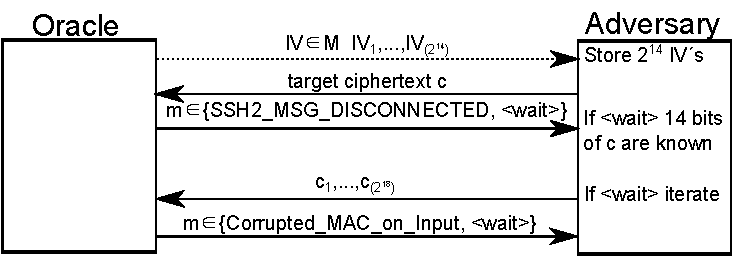
\includegraphics[scale=1]{drawing.pdf}
	\caption{Attack on the SSH BPP protocol~\cite{Albrecht2009}}
	\label{fig:BPPAttack}
\end{figure*}



\section{Alternatives}
\indent Bellare et al.~\cite{Bellare2004} propose a few alternatives to the BPP protocol. SSH-NPC, SSH-\$NPC, SSH-CTR, SSH-CTRIVCBC and SSH-EIV-CBC.
\indent SSH-NPC and SSH-\$NPC (No Packet Chaining) use CBC mode with random per packet IV's~\cite{Albrecht2009}. Albrecht et al show that using these alternatives won't matter as long as the attacker can still distinguish between a packet-length check failure and a MAC failure. The attacker can just inject a random IV block, instead of using the last packet's last ciphertext block.

\indent Furthermore, control over the IV gives an attacker more advantages. For example, he can distinguish whether a message $M_1$ or message $M_2$ was encrypted.

% Insert small security game here

\indent Albrecht et al. show that SSH-CTR, SSH-CTRIVCBC and SSH-EIV-CBC are resistant to their attack. SSH-CTR because it uses a counter mode. SSH-CTRIVCBC and SSH-EIV-CBC because the attacker is unable to see the IV since it is either the encryption of a counter or encipherment of the last ciphertext block.

\indent OpenSSH 5.2 switched to AES counter mode, but currently no SSH implementations use either SSH-CTRIVCBC or SSH-EIV-CBC.

\section{Countermeasures}
\indent One of the countermeasures OpenSSH took was to return the same error message when either the length check or the block-length check failed. By not having this distinction, an attacker can't apply the first attack to reveal the first 14 bits. However this doesn't prevent the 32-bit recovery attack. An extra improvement is to randomize the length field if the length check fails. The system then proceeds with the new length until the MAC check fails. This will causes a problem for our attacker since it now doesn't know if the length is accepted and the MAC tag just failed or the length isn't accepted and it just returns the MAC error.

\section{Conclusion}
It is possible to recover plaintext bits from a proven secure SSH implementation. Therefore it is also hard to know whether improvements to resolve this issue won't lead to new attacks on these SSH implementations.
\bibliography{Master}



\end{document}